
\documentclass[ aspectratio=169 ]{beamer}

% Pakiety
\usepackage[utf8]{inputenc}
\usepackage[T1]{fontenc}
\usepackage[polish]{babel}
\usepackage{graphicx}
\usepackage{amsmath}
\usepackage{tikz}

% Motyw prezentacji
\usetheme{Madrid}
\usecolortheme{default}

% Informacje o prezentacji
\title{Algorytmy i ich zastosowania}
\subtitle{Wprowadzenie do świata algorytmiki}
\author{Autor prezentacji}
\institute{Projekt Prezentacja}
\date{\today}

\begin{document}

% SLIDE 1 - Slajd tytułowy
\begin{frame}
    \titlepage
\end{frame}

% SLIDE 2 - Spis treści
\begin{frame}
    \frametitle{Spis treści}
    \tableofcontents
\end{frame}

\section{Podstawy algorytmów}

% SLIDE 3 - Definicja algorytmu
\begin{frame}
    \frametitle{Czym jest algorytm?}

    Algorytm to uporządkowany zestaw instrukcji prowadzących
    do rozwiązania określonego problemu.

    \begin{block}{Najważniejsze cechy algorytmu}
        \begin{itemize}
            \item Jednoznaczność instrukcji.
            \item Określona kolejność działań.
            \item Skończona liczba kroków.
            \item Możliwość uzyskania wyniku.
        \end{itemize}
    \end{block}

    \begin{alertblock}{Ważne!}
        Algorytm powinien prowadzić do poprawnego rozwiązania
        problemu w skończonym czasie.
    \end{alertblock}
\end{frame}

% SLIDE 4 - Rodzaje algorytmów
\begin{frame}
    \frametitle{Rodzaje algorytmów}

    Możemy wyróżnić kilka podstawowych rodzajów algorytmów:

    \begin{enumerate}
        \item Algorytmy sortowania.
        \item Algorytmy wyszukiwania.
        \item Algorytmy rekurencyjne.
        \item Algorytmy grafowe.
    \end{enumerate}

    \begin{exampleblock}{Przykład}
        Sortowanie liczb od najmniejszej do największej
        jest przykładem algorytmu sortowania.
    \end{exampleblock}
\end{frame}

\section{Działanie algorytmów}

% SLIDE 5 - Przykład działania
\begin{frame}
    \frametitle{Jak działa algorytm?}

    Przykład: algorytm obliczający sumę dwóch liczb.

    \begin{block}{Kolejne kroki}
        \begin{enumerate}
            \item Pobierz pierwszą liczbę.
            \item Pobierz drugą liczbę.
            \item Dodaj obie liczby.
            \item Wyświetl wynik.
        \end{enumerate}
    \end{block}

    \[
        S = a + b
    \]

    Dla $a=5$ i $b=7$ otrzymujemy:

    \[
        S = 5+7=12
    \]
\end{frame}

% SLIDE 6 - Złożoność obliczeniowa
\begin{frame}
    \frametitle{Złożoność obliczeniowa}

    Złożoność obliczeniowa określa ilość zasobów potrzebnych
    do wykonania algorytmu.

    \begin{block}{Notacja Big O}
        Pozwala opisać tempo wzrostu czasu działania algorytmu.
    \end{block}

    Przykładowe złożoności:

    \begin{itemize}
        \item $O(1)$ -- stała.
        \item $O(\log n)$ -- logarytmiczna.
        \item $O(n)$ -- liniowa.
        \item $O(n^2)$ -- kwadratowa.
    \end{itemize}

    \[
        T(n)=O(n)
    \]
\end{frame}

% SLIDE 7 - Dwie kolumny
\begin{frame}
    \frametitle{Algorytmy sortowania}

    \begin{columns}

        \column{0.48\textwidth}
        \begin{block}{Sortowanie bąbelkowe}
            \begin{itemize}
                \item Porównuje sąsiednie elementy.
                \item Zamienia je miejscami.
                \item Powtarza operację.
            \end{itemize}
            Złożoność:
            \[
                O(n^2)
            \]
        \end{block}

        \column{0.48\textwidth}
        \begin{block}{Sortowanie szybkie}
            \begin{itemize}
                \item Wybiera element bazowy.
                \item Dzieli zbiór na części.
                \item Sortuje podzbiory.
            \end{itemize}
            Średnia złożoność:
            \[
                O(n\log n)
            \]
        \end{block}

    \end{columns}
\end{frame}

\section{Zastosowania algorytmów}

% SLIDE 8 - Grafika
\begin{frame}
    \frametitle{Grafika przedstawiająca algorytmy}

    Algorytmy są wykorzystywane w wielu dziedzinach
    informatyki i codziennego życia.

    \begin{center}
        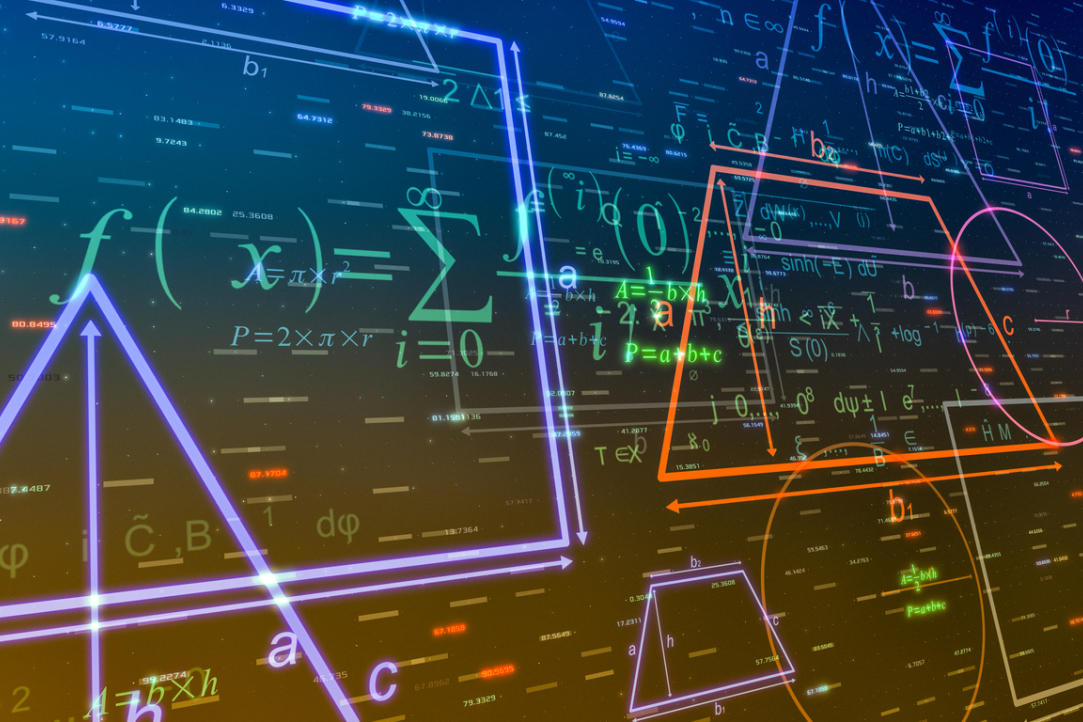
\includegraphics[width=0.75\textwidth,height=0.55\textheight,
        keepaspectratio]{Algorithms.jpg}
    \end{center}

    \begin{exampleblock}{Przykład zastosowania}
        Algorytmy wyszukiwania pomagają znaleźć informacje
        w dużych zbiorach danych.
    \end{exampleblock}
\end{frame}

% SLIDE 9 - Zastosowania
\begin{frame}
    \frametitle{Gdzie wykorzystujemy algorytmy?}

    \begin{itemize}
        \item \textbf{Medycyna} -- analiza danych i obrazów.
        \item \textbf{Transport} -- wyznaczanie najkrótszych tras.
        \item \textbf{Internet} -- wyszukiwarki i rekomendacje.
        \item \textbf{Bankowość} -- analiza transakcji.
        \item \textbf{Sztuczna inteligencja} -- uczenie maszynowe.
    \end{itemize}

    \begin{alertblock}{Znaczenie algorytmów}
        Bez algorytmów wiele współczesnych technologii
        nie mogłoby działać tak sprawnie.
    \end{alertblock}
\end{frame}

% SLIDE 10 - Podsumowanie
\begin{frame}
    \frametitle{Podsumowanie}

    \begin{block}{Najważniejsze informacje}
        \begin{enumerate}
            \item Algorytmy rozwiązują określone problemy.
            \item Składają się z uporządkowanych instrukcji.
            \item Mogą mieć różną złożoność obliczeniową.
            \item Są podstawą działania programów komputerowych.
        \end{enumerate}
    \end{block}

    \begin{center}
        \Large \textbf{Dziękuję za uwagę!}
    \end{center}

\end{frame}

\end{document}
